\documentclass{article}

\usepackage{graphicx}
\usepackage{rotating} % support sidewaystable
\usepackage{listings}
\lstset{
  breaklines=true,
  basicstyle=\ttfamily,
}

\title{Experimental Report: A Prove of Concept Implementation of Networking for CreamFL}
\author{Xie Yu Guang}
\date{\today}

\begin{document}

\maketitle

\section{Introduction}
The purpose of this report is to present the results of modifying CreamFL\cite{yu2023multimodal} to run in an distributed faction. The report will provide details of replicating the results of running CreamFL using centralized and distributed execution. The goal is prove that the refactored code supports running CreamFL in a federated learning environment. 

\section{Experimental Setup}

\subsection{Hardware}
Because of limited resources, the experiment was conducted on a single machine. The machine has 6 cores, 16GB of RAM and a single NVIDIA GeForce GTX 1050 Ti. As such, fulling replicating the results of the original paper is not possible. Instead, we will run smaller experiments that require a smaller communication/memory size and compute power.

\subsection{Software modifications}
To allow fast development cycles, we first modified the code base to allow easy limiting client training data size by adding a "--max-size" flag. 

A bug was also fixed in the code base where training crashed when a type of client was configured but not selected for training in a round, this bug was more prominent with few clients. 

The random initialization process has been fixed to enable identical runs to utilize a predefined random seed set in the flag. An debugging line was left in the original code to always set the seed to 2021. Additionally, it can now operate with a random seed. If the seed is set to 0, the system defaults to a random seed, which is determined based on the current time. In this case, the \texttt{cudnn.deterministic} attribute is set to \texttt{False}, and \texttt{cudnn.benchmark} is set to \texttt{True} as a performance improvement.

This setup of setting the seed to current time is used in all the experiments in this report. This is because the pass of execution is different in the centralized and distributed runs. Instead of comparing the results of two runs for equality, which is not expected to work. We can only comparing the results of two distributions for equality by running each setup multiple times.

\subsection{Distributed Architecture}
The distributed architecture is split to three main components: the state server, the clients, and the global model computation provider. The server is responsible for sending the learned features to the clients and collecting the results. The clients are responsible for client side training and sending the results back to the server. The global model computation provider is responsible for computing the global model from the results of the clients, computing the learned features, and evaluating the global model

We split the server into a state reporting server and a model computation provider. This is mainly because of the single threaded nature of python would otherwise make the server non-responsive when the model computation is running. 

The clients and global model only communicate with the server and each other over http and file io. The http server uses json and client wait for updates by polling the server in regular intervals. Features are shared between the clients and the global model computation provider using files and never uploaded to the server. However, the server distributes hashes of the features that is use to find the feature files. This design can be easily extended to use a CDN.

\subsection{Client Training Data}
To keep the experiment as close as possible to the original code base. The client training data is generated using the same method as the original code base, including how the data is loaded on to the client. Both the centralized and distributed client use the same data splitting indexes, when testing under the same parameters.

In a real world scenario, each client would have their own data. We skipped this step to simplify the experimental setup, at a slight cost to client start up time, where all data is loaded and only the data indexed are kept. We expect different real world scenarios to require different data preparation and loading methods. There for, build one just for this experiment is not worth the cost.


\section{Results and Analysis}
% Present the results obtained from the experiment and analyze them. Discuss the task convergence, model effect, and any other observations or insights.

\begin{figure}[ht]
    \centering
    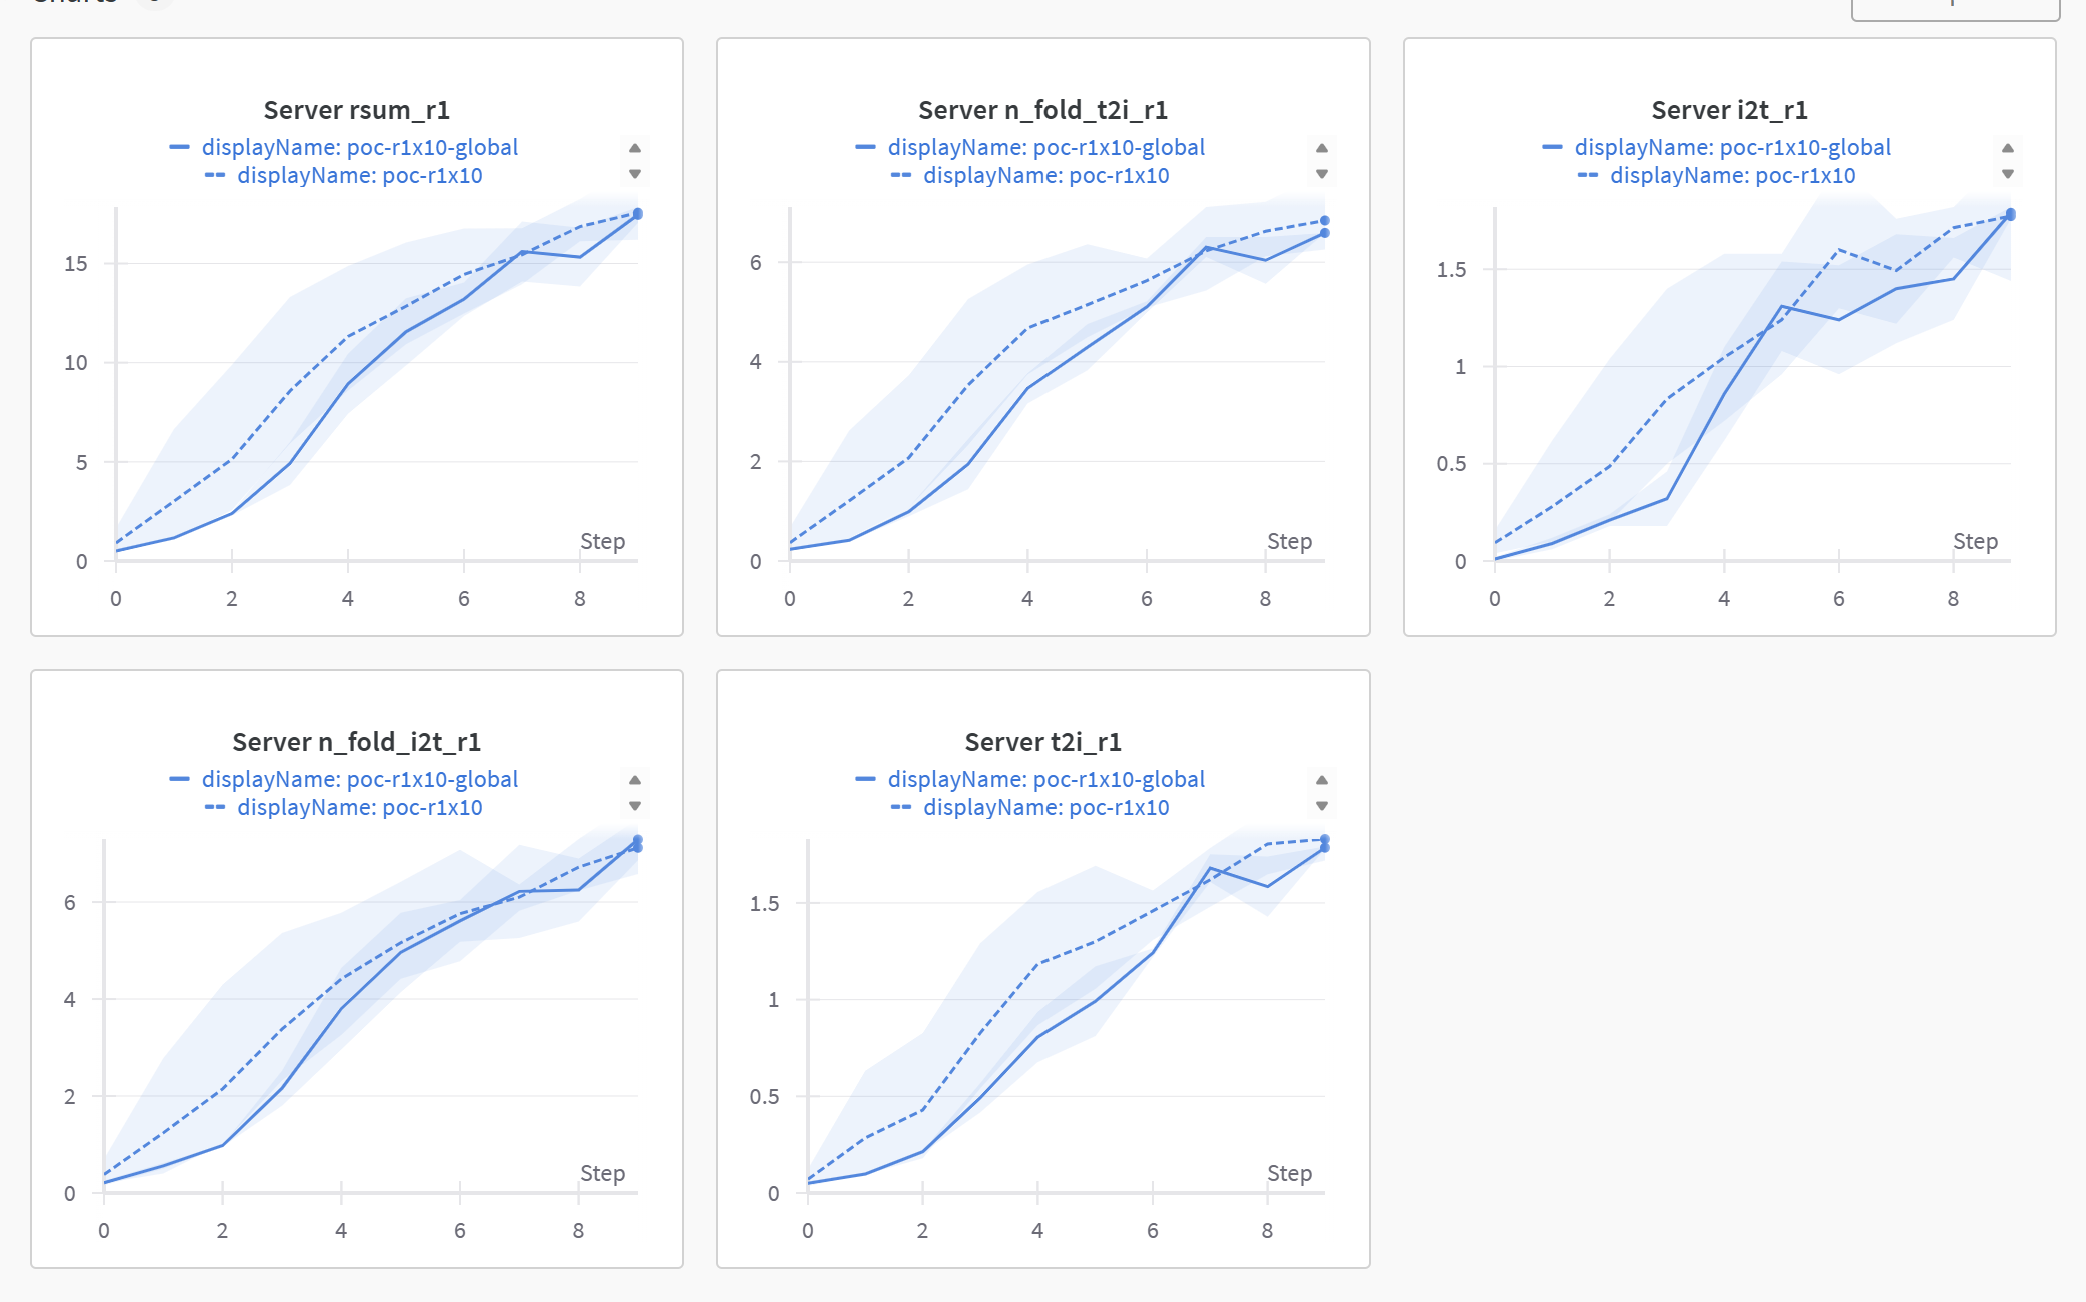
\includegraphics[width=0.8\textwidth]{poc-r1x10.png}
    \caption{Train with 1 client over 10 communication rounds. "poc-r1x10" are centralized runs and "poc-r1x10-global" are distributed runs.}
    \label{fig:r1x10}
\end{figure}

In Figure \ref{fig:r1x10}, the parameters used were: 
\begin{lstlisting}
    --contrast_local_inter --contrast_local_intra 
    --interintra_weight 0.5 --max_size 50000 
    --pub_data_num 4000 --feature_dim 64 
    --num_img_clients 0 --num_txt_clients 1 
    --num_mm_clients 0 --client_num_per_round 1 
    --local_epochs 5 --comm_rounds 10 --not_bert 
    --seed 0
\end{lstlisting}

This was run 3 times centralized and 2 times distributed to compare the performance of the two. The graph shows that the model performance become highly varied in the first few communication rounds, but coverages to similar results at the end. The end results are shown in Table \ref{table:r1x10}.

\begin{sidewaystable}
    \centering
    \begin{tabular}{|l|l|l|l|l|l|l|l|}
    \hline
    Name & Runtime & ID & i2t\_r1 & n\_fold\_i2t\_r1 & n\_fold\_t2i\_r1 & rsum\_r1 & t2i\_r1 \\
    \hline
    poc-r1x10-global & 5.9h\footnote{computer went to sleep} & 9eebn4qd & 1.82 & 6.86 & 6.588 & 17.06 & 1.792 \\
    poc-r1x10-global & 2.3h & goljw32i & 1.76 & 7.72 & 6.588 & 17.848 & 1.78 \\
    poc-r1x10 & 2.2h & 3u0urus7 & 1.76 & 6.66 & 6.256 & 16.408 & 1.732 \\
    poc-r1x10 & 2.0h & bkiu5ffi & 2.12 & 8.12 & 7.804 & 20.084 & 2.04 \\
    poc-r1x10 & 2.0h & 0g6ia4ds & 1.44 & 6.58 & 6.452 & 16.192 & 1.72 \\
    \hline
    \end{tabular}
    \caption{Comparing the results of centralized vs distributed inference with 1 client over 10 communication rounds. The "poc-r1x10" are centralized runs and "poc-r1x10-global" are distributed runs. The runtime is the time taken to complete the experiment. The ID is the experiment id, this id can be appended to <https://wandb.ai/xiegeo/CreamFL/runs/> to view the experiment details. The rest of the columns are the results of the experiment.}
    \label{table:r1x10}
\end{sidewaystable}


\section{Future Work}

There are many possible improvements that can be made, both to the code base and the experimental setup. Capable of fulling replicating the results of the original paper is ideal.

However, for the interest of usability and long time support, perhaps we should also turn to another direction ---\ wrapping CreamFL as a component of an established federated learning framework, such as FATE or FedML. This would save us from reinventing the wheel and allow existing users of these frameworks to easily integrate CreamFL as a component of their federated learning system.

\section{Conclusion}
% Summarize the findings of the experiment and draw conclusions about the effectiveness of the distributed framework.

The results of the experiment show that the distributed framework is capable of running CreamFL. However, due to the limited resources the results are not as conclusive as we would like. 

\bibliography{poc}
\bibliographystyle{plain}

\end{document}